%%%%%%%%%%%%%%%%%%%%%%%%%%%%%%%%%%%%%%%%%
% 
% LaTeX Template
% Version 3.1 (25/3/14)
%
%%%%%%%%%%%%%%%%%%%%%%%%%%%%%%%%%%%%%%%%%

%----------------------------------------------------------------------------------------
%	PACKAGES AND DOCUMENT CONFIGURATIONS
%----------------------------------------------------------------------------------------

\documentclass[12pt, a4 paper]{article}

\usepackage{tikz}
%\usepackage[top=2cm, bottom=2cm, outer=0cm, inner=0cm]{geometry}
\usepackage{graphicx} % Required for the inclusion of images
\usepackage{multicol} % Required for multicolumns
\usepackage{setspace} % Required for line spacing
\setlength\parindent{0pt} % Removes all indentation from paragraphs
\setlength{\columnseprule}{0.4pt} % Adds vertical line between multicolumns
\usepackage{multirow} % Required for multirows
\usepackage{booktabs} % For prettier tables
\usepackage{xcolor}
%\usepackage{tabularx}
%\renewcommand{\rmdefault}{ptm}

%\usepackage{helvet}

\usepackage{times} % Uncomment to use the Times New Roman font

%----------------------------------------------------------------------------------------
%	DOCUMENT INFORMATION
%----------------------------------------------------------------------------------------

\begin{document}

\tikz[remember picture,overlay] \node[inner sep=0pt] at (current page.center){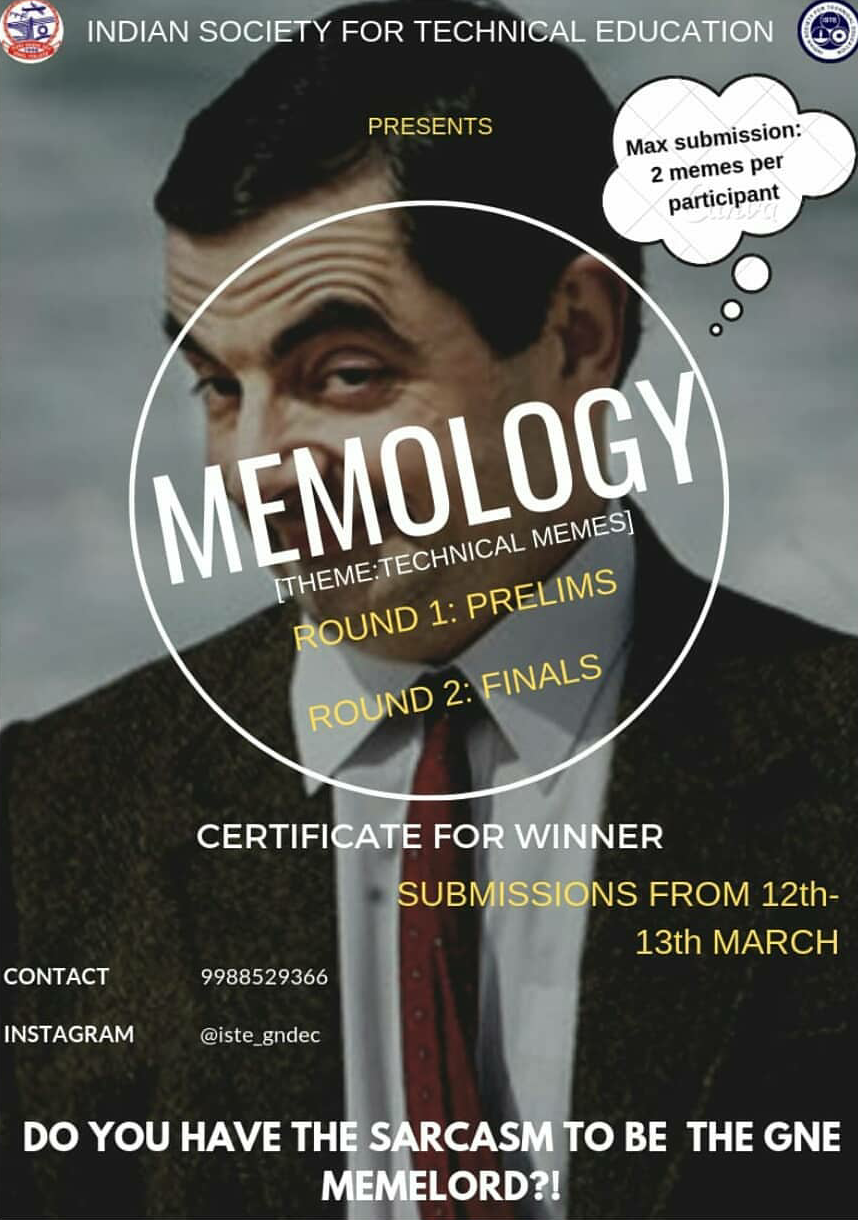
\includegraphics[width=\paperwidth,height=\paperheight]{image.png}};

\clearpage

%\font\myfont=cmr12 at 35pt
%\title{\myfont  Event Name} % Write Event name here
%\author{}
%\date{\vspace{-10ex}}

%\maketitle % Insert the title, author and date
\setstretch{1.5}

%\tikz[remember picture,overlay] \node[opacity=0.8,inner sep=0pt] at (current page.center){
\includegraphics[width=\paperwidth,height=\paperheight]{Border48-A4--Arvin61r58.png}};
%\tikz[remember picture,overlay] \node[opacity=0.5,inner sep=0pt] at (current page.center){\includegraphics[width=\paperwidth,height=\paperheight]{color-2174049__340.png}};

\begin{center}
\Huge \bfseries \ttfamily MEMOLOGY
\end{center}

\begin{center}
\large An online event to find Memelord
\end{center}

\begin{center}
\begin{multicols}{2}
\begin{tabular}{l r}
Date: & March 12-18\\ % Date the event was held
%Time: & X pm to Y pm \\ % Time of event 
\end{tabular}
\columnbreak
\begin{tabular}{l r}
Venue: & Instagram \\ % Venue of event
%Total Attendance: & Number \\ % Number of participants
\end{tabular}
\end{multicols}


\begin{LARGE}
Prelims  and  Finals
\end{LARGE}

\begin{Large}
\begin{multicols}{2}
Inspire the art of meme making
An online event “MEMOLOGY” was organized from march 12 to march 18, 2019 on Instagram handle $@$istegndec. 
\columnbreak
%\includegraphics[width=\linewidth]{placeholder.jpg}
  %\caption{A boat.}
  %\label{fig:boat1}
\end{multicols}

\begin{multicols}{2}

%\includegraphics[width=\linewidth]{placeholder.jpg}

\columnbreak
Basically, the event was to take submissions based on a theme from participants and evaluate them on basis of public response. The event consisted of 2 rounds.
\end{multicols}

\newpage 

%\tikz[remember picture,overlay] \node[opacity=0.8,inner sep=0pt] at (current page.center){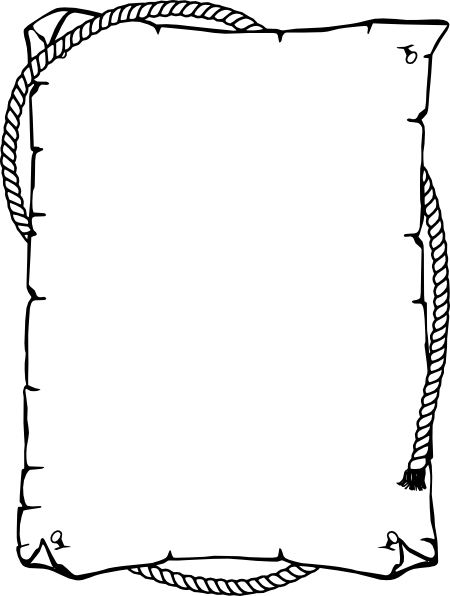
\includegraphics[width=\paperwidth,height=\paperheight]{5TRrp44jc.png}};
%\tikz[remember picture,overlay] \node[opacity=0.8,inner sep=0pt] at (current page.center){\includegraphics[width=\paperwidth,height=\paperheight]{md_5b0912b7c0870.png}};

\begin{multicols}{2}
First round included posting the received submissions in groups of 5 on Instagram by allotting every meme a unique code. 
\columnbreak
%\includegraphics[width=\linewidth]{placeholder.jpg}
  
\end{multicols}

\begin{multicols}{2}
%\includegraphics[width=\linewidth]{placeholder.jpg}

\columnbreak
The audience was supposed to comment the code of the meme they liked the most. We received 500+ comments in round 1 which was a record-breaking response.
  
\end{multicols} 

\begin{multicols}{2}
In Second round, the meme with top votes in each group in first round qualified.  The qualified memes were posted individually and evaluation was done on basis of public likes.

\columnbreak
%\includegraphics[width=\linewidth]{placeholder.jpg}
  
\end{multicols} 

\begin{multicols}{2}
%\includegraphics[width=\linewidth]{placeholder.jpg}

\columnbreak
 The meme with the most likes was declared the winner.
  
\end{multicols} 

\end{Large} 
\end{center}

\newpage 

%\tikz[remember picture,overlay] \node[opacity=0.8, inner sep=0pt] at (current page.center){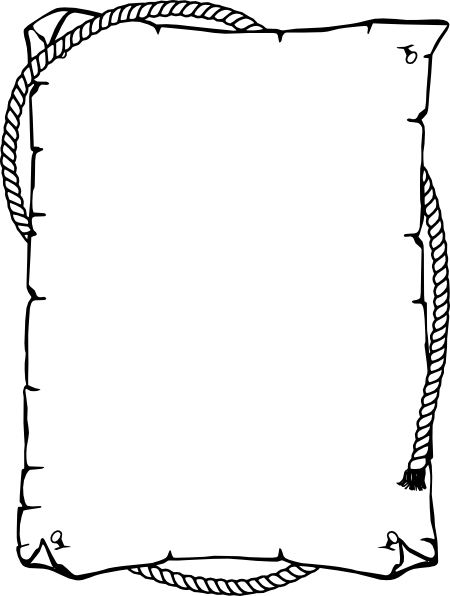
\includegraphics[width=\paperwidth,height=\paperheight]{5TRrp44jc.png}};
%\tikz[remember picture,overlay] \node[opacity=0.8,inner sep=0pt] at (current page.center){\includegraphics[width=\paperwidth,height=\paperheight]{md_5b0912b7c0870.png}};

\begin{center}
\Huge Pictures Section
\end{center}

\newpage 

\tikz[remember picture,overlay] \node[opacity=0.8,inner sep=0pt] at (current page.center){
\includegraphics[width=\paperwidth,height=\paperheight]{image1.jpeg}};

\newpage

\tikz[remember picture,overlay] \node[opacity=0.8,inner sep=0pt] at (current page.center){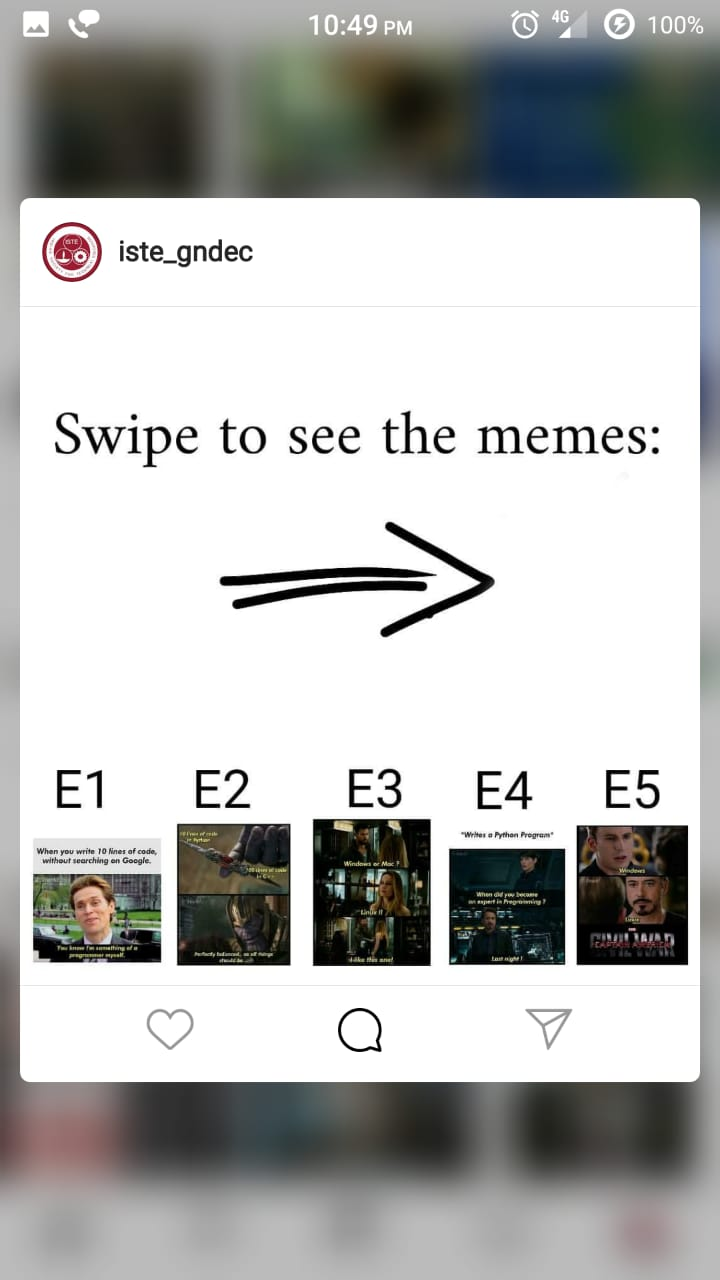
\includegraphics[width=\paperwidth,height=\paperheight]{image2.jpeg}};


\newpage 

\tikz[remember picture,overlay] \node[opacity=0.8,inner sep=0pt] at (current page.center){
\includegraphics[width=\paperwidth,height=\paperheight]{image4.jpeg}};

\newpage

\tikz[remember picture,overlay] \node[opacity=0.8,inner sep=0pt] at (current page.center){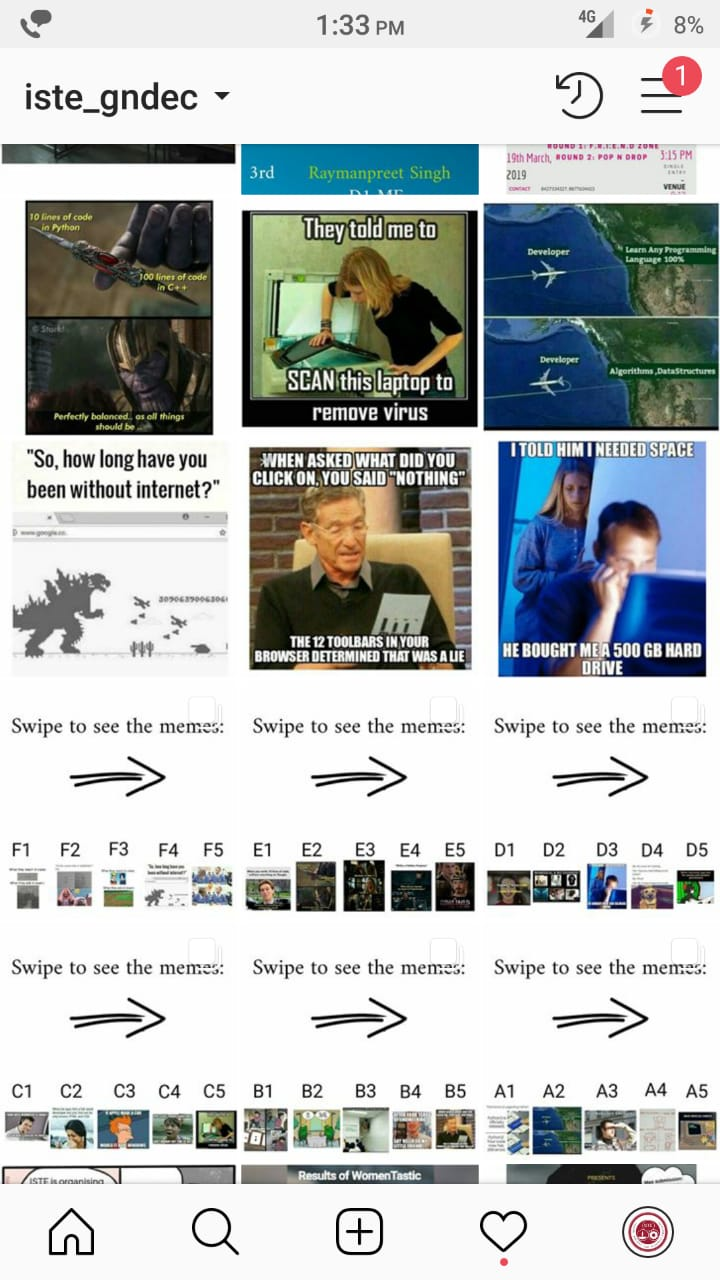
\includegraphics[width=\paperwidth,height=\paperheight]{image6.jpeg}};

\newpage

\begin{center}
\huge Organisers list
\end{center}

\begin{table}[h!]
  \begin{center}
    \begin{tabular}{|c|c|c|c|c|c|} 
    \toprule % <-- Toprule here
      \textbf{S.No.} & \textbf{Name} & \textbf{Branch/Year} & \textbf{Roll NO.} \\
      \midrule % <-- Midrule here
      1 & Jagmeet Singh        & D2 ECE & 1706728 \\
      2	& Tushar Chauhan       & D2 ME	& 1706533 \\
      3	& Dilnish Kaur Bagga   & D2 ECE	& 1706721 \\
      4	& Ishpreet Kaur Gulati & D2 CSE	& 1706443 \\
      5	& MANSIMAR SINGH	   & D1 IT	& 1805527 \\
      6	& Parneet Kaur	       & D2 CSE & 1706486 \\
      7	& Pawandeep Singh	   & D4 CSE	& 1507637 \\
      8	& Kanishka Malhotra	   & D1 IT	& 1816050 \\

      \bottomrule % <-- Bottomrule here
    \end{tabular}
  \end{center}
\end{table}

\newpage

\tikz[remember picture,overlay] \node[opacity=0.8,inner sep=0pt] at (current page.center){
\includegraphics[width=\paperwidth,height=\paperheight]{image3.jpeg}};

\newpage

\tikz[remember picture,overlay] \node[opacity=0.8,inner sep=0pt] at (current page.center){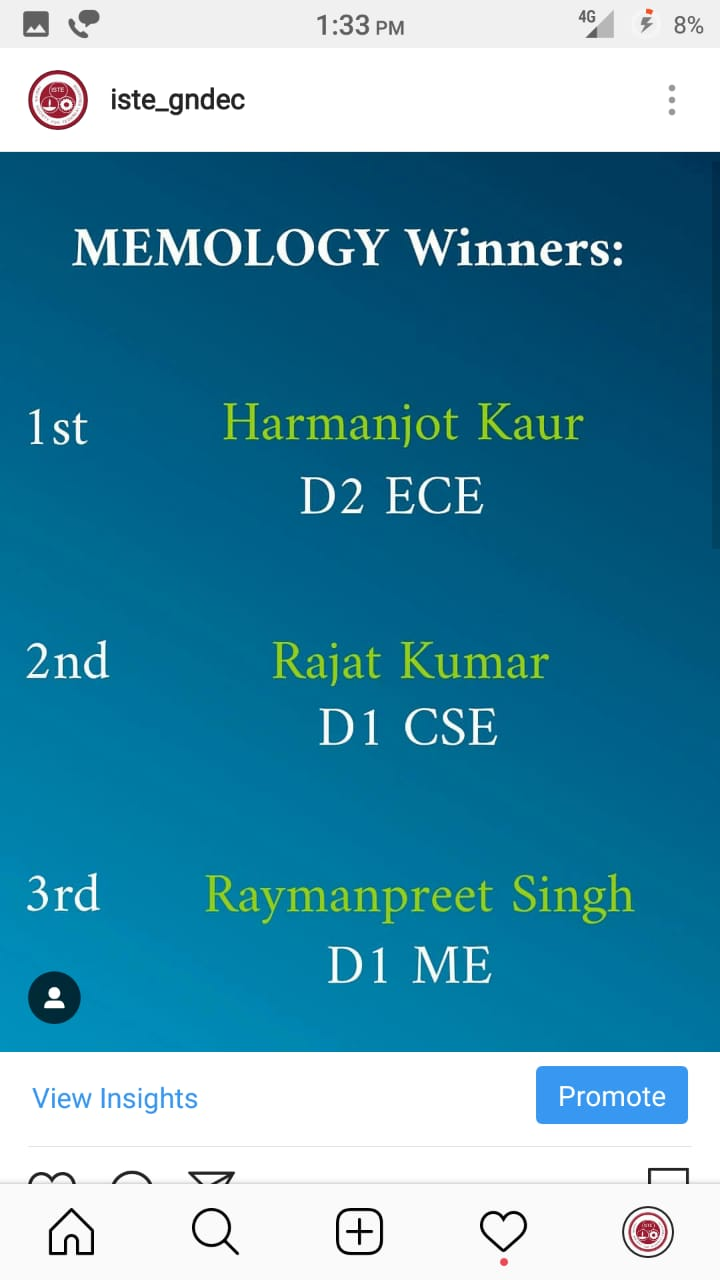
\includegraphics[width=\paperwidth,height=\paperheight]{image5.jpeg}};

\newpage

\begin{center}
\huge Winners List
\end{center}

\begin{table}[h!]
  \begin{center}
    \begin{tabular}{|c|c|c|c|c|c|} 
    \toprule % <-- Toprule here
      \textbf{S.No.} & \textbf{Name} & \textbf{Branch/Year} & \textbf{Roll No.} &\textbf{Position} \\
      \midrule % <-- Midrule here
      1 & Harmanjot Kaur 	& ECE D2 & 1706728 & 1st \\
      2	& Rajat Kumar	    & CSE D1 & 1805214 & 2nd \\
      3	& Raymanpreet Singh & ME  D1 & 1805701 & 3rd \\

      \bottomrule % <-- Bottomrule here
    \end{tabular}
  \end{center}
\end{table}

\begin{center}
\huge Participant list
\end{center}

\begin{table}[h!]
  \begin{center}
    \begin{tabular}{|c|c|c|c|c|c|} 
    \toprule % <-- Toprule here
      \textbf{S.No.} & \textbf{Name} & \textbf{Branch/Year } &\textbf{Year/Branch}\\
      \midrule % <-- Midrule here
      1	 & Jagdeep Gill	           & IT	 D2 & 1819968 \\
      2	 & Harmanjot Kaur	       & ECE D2	& 1706728 \\
      3	 & Rajat Kumar	           & CSE D1	& 1805214 \\
      4	 & Raymanpreet Singh	   & ME	 D1	& 1805701 \\
      5	 & Adarsh Ranjan	       & CSE D1	& 1815103 \\
      6	 & Ritu	                   & ECE D1	& 1817070 \\
      7	 & Sudhanshu Dubey	       & CSE D2	& 1706523 \\
      8	 & Shahbaz Singh Sammewali & CSE D1	& 1805225 \\
      9	 & Aman Chauhan	           & CSE D1	& 1805158 \\
      10 & Satinder Singh Saini	   & CSE D1	& 1805223 \\
      11 & Jagjit Singh	           & CSE D1	& 1815031 \\
      12 & Ravi Mittal	           & CSE D4	&         \\
      13 & Prashant Singh	       & PE	 D4	&         \\

      \bottomrule % <-- Bottomrule here
    \end{tabular}
  \end{center}
\end{table}


\end{document}